%! Author = nico 
%! Date = 17.06.23

\section{Bausteinsicht}
\label{sec:bausteinsicht}

\subsection{Systemübersicht}
\label{subsec:systemuebersicht}
Das System ist in Microservices unterteilt. Jeder Microservice hat eine eigenständige Aufgabe und ist für diese verantwortlich. Es findet keine Kommunikation unter den Microservices statt, da alle Microservices auf ein und dieselbe Datenbank zugreifen.
Die Kommunikation mit dem Frontend findet über eine REST-API zum jeweiligen Microservice statt. Die einzelnen Microservices sind in Abbildung \ref{fig:systemuebersicht} dargestellt.

\begin{figure}[H]
    \centering
    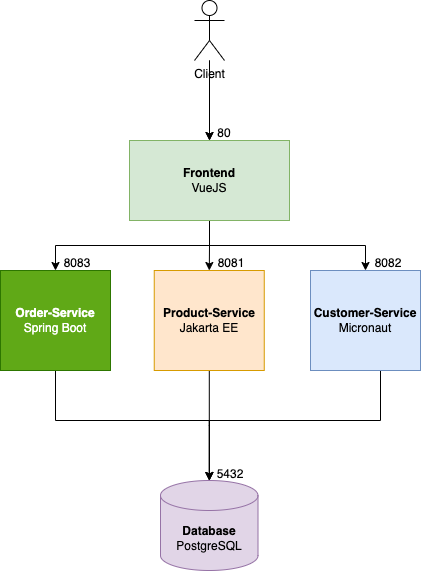
\includegraphics[width=0.5\textwidth]{../images/bausteinsicht/systemarchitektur.png}
    \caption{Systemübersicht}
    \label{fig:systemuebersicht}
\end{figure}

\subsection{Schichtensicht}
\label{subsec:schichtensicht}
Jeder Microservice ist gleich aufgebaut. Es gibt eine REST-API pro Microservice, welche die Kommunikation mit dem Frontend ermöglicht. Die REST-API kommuniziert jeweils mit dem Controller, welcher die Anfrage entgegennimmt und verarbeitet. Der Controller kommuniziert anschliessend mit dem Service-Layer, welcher die Business-Logik enthält. Der Service-Layer macht dann die nötigen Anfragen zum Repository-Layer, welcher die Datenbankzugriffe enthält. Die Schichten sind in Abbildung \ref{fig:schichtensicht} dargestellt.

\begin{figure}[H]
    \centering
    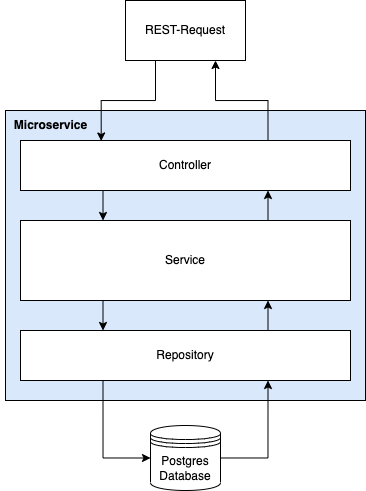
\includegraphics[width=0.6\textwidth]{../images/bausteinsicht/schichtensicht.png}
    \caption{Schichtensicht}
    \label{fig:schichtensicht}
\end{figure}

\subsection{Klassen- und Paketsicht}
\label{subsec:klassen-und-paketsicht}
Nachfolgend sind alle Klassen zu sehen, die in den Microservices verwendet werden. Wichtig zu bemerken ist, dass nicht jeder Microservice jede dieser Klassen hat. Sie wurden nur zusammengeführt, um eine Übersicht über die Datenstruktur
zu ermöglichen. Daher kommt auch, dass nicht alle Klassen andere Klassen sauber referenzieren, bei \texttt{Order} zum Beispiel ist der \texttt{Customer} nur via ID referenziert, genauso bei \texttt{BeerOrder} die Klasse \texttt{Beer}.
\begin{figure}[H]
    \centering
    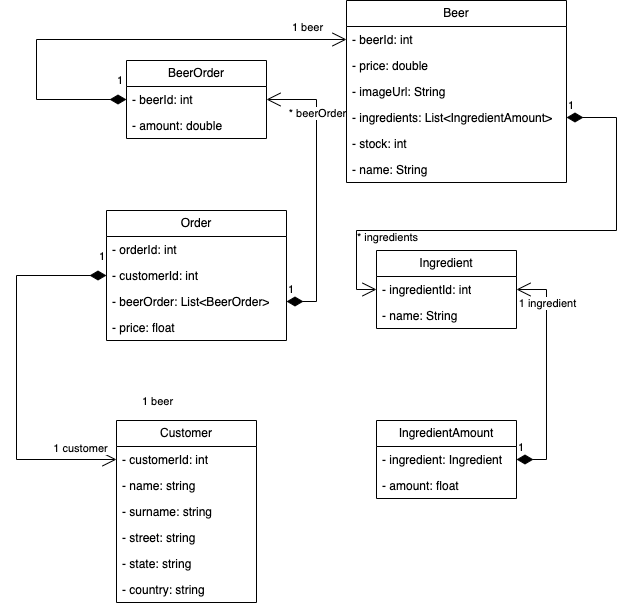
\includegraphics[width=0.6\textwidth]{../images/bausteinsicht/klassendiagramm.png}
    \caption{Klassendiagramm}
    \label{fig:klassendiagramm}
\end{figure}

\subsection{Entity Relationship Modell}
\label{subsec:entity-relationship-modell}
Wie in Abbildung \ref{fig:entityrealationshipmodell} dargestellt, gibt es insgesamt 6 Entitäten. Die Tabellen \texttt{BeerOrder} und \texttt{BeerIngredient} sind Zwischentabellen, da es zwischen den jeweiligen Typen eine n:m Beziehung gibt. Die Entitäten \texttt{Beer}, \texttt{Ingredient} und \texttt{Order} sind die Hauptentitäten. \texttt{Beer} enthält die Biersorten sowie den aktuellen Lagerbestand. \texttt{Ingredient} enthält die Zutaten, welche in den Biersorten enthalten sind. Und \texttt{Order} enthält die Bestellungen, welche aufgegeben werden. Die Entitäten sind in Abbildung \ref{fig:entityrealationshipmodell} dargestellt.

\begin{figure}[H]
    \centering
    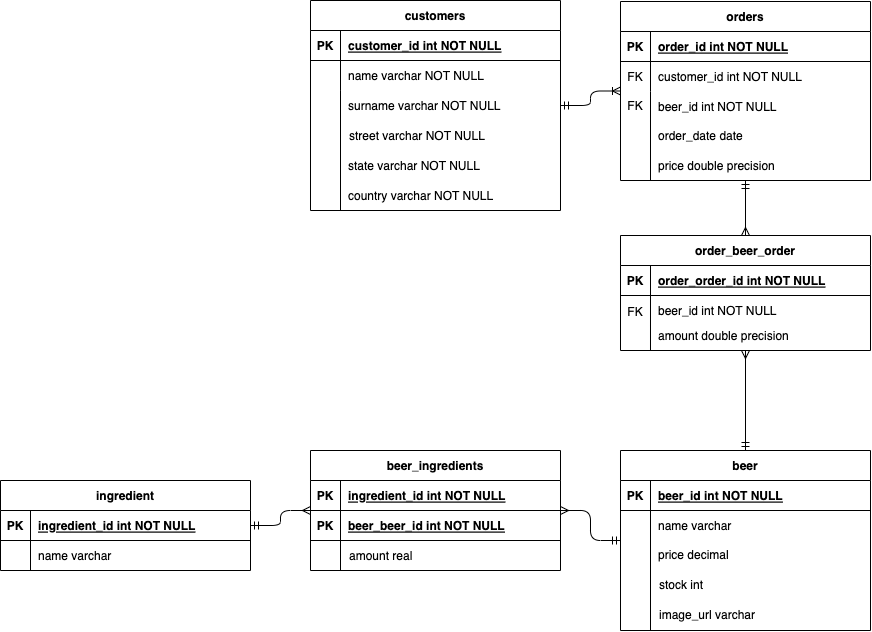
\includegraphics[width=0.7\textwidth]{../images/bausteinsicht/erm.png}
    \caption{Entity Relationship Modell}
    \label{fig:entityrealationshipmodell}
\end{figure}

\subsection{Services}
\label{subsec:Services}
In diesem Kapitel werden grob die einzelnen Services, das Frontend sowie die Datenbank beschrieben.
Die Schnittstellenbeschreibung für jeden Service werden separat in der API-Dokumentation beschrieben.

\subsubsection{Datenbank mit Docker Compose}
\label{subsec:datenbank-docker}
Die Postgres-Datenbank wird in Docker gestartet.
Dies hat den Vorteil, dass lokal nichts aufgesetzt werden muss und die
Datenbank einfach zurückgesetzt werden kann.
In der Datei \texttt{docker-compose.yml} befindet sich die Konfiguration der Datenbank.


\subsubsection{Frontend}
\label{subsubsec:Frontend}
Das Frontend ist die Schnittstelle zwischen dem Benutzer und dem System. Als Frontend wird VueJS verwendet. VueJS ist ein JavaScript Framework, welches auf dem Model-View-ViewModel (MVVM) Pattern basiert. Der Aufbau des Frontends ist in Abbildung \ref{fig:frontend} dargestellt.

Das Frontend ist modular und in Komponenten unterteilt. Im Zentrum des Frontend stehen die Komponenten
in der Router View. Die Router View umschliesst alle Komponenten und wird in der App eingebunden. In der
App befindet sich nebst der Router View noch die Navigation. Somit ist die Navigation von jeder Seite aus
sichtbar.
Der Router verwaltet die einzelnen Views und bestimmt, auf welche View der Benutzer weitergeleitet wird.
Pinia ist der zentrale Store des Frontends. In Pinia werden die Daten gespeichert, welche von den Komponenten verwendet werden.

\begin{figure}[H]
    \centering
    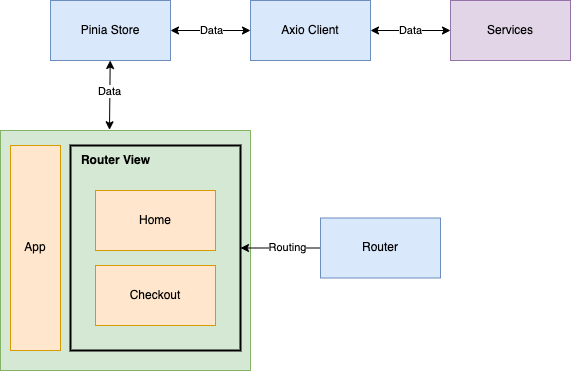
\includegraphics[width=0.7\textwidth]{../images/bausteinsicht/frontend.png}
    \caption{Frontend Architektur Sicht}
    \label{fig:frontend}
\end{figure}

In der Router-View werden zwei Views abgebildet: In der Home-View sind die Biersorten sichtbar und es ist der Einstiegspunkt der Applikation. In der Checkout-View kann der Benutzer seine Bestellung mit Angabe seiner Daten abschliessen.
Die App-View beinhaltete die Router-View, sowie die Navigation und ist somit die Hauptkomponente des Frontends. 


\subsubsection{Product Service}
\label{subsubsec:ProductService}
Der Product Service beinhaltet die Logik für die Verwaltung der Biersorten. Dieser Service ist in Jakarta EE geschrieben. Der Service ist sehr simpel und es können dort lediglich Biersorten und wie viele davon vorhanden sind, verwaltet werden.

\paragraph{Datenbank Verbindung} \mbox{} \\ 
Die Datenbankverbindung wird in der Datei \texttt{src/resources/META-INF/persistence.xml} konfiguriert.
Dort werden die Angaben zur Verbindung gemacht: der Host, der Port, der Name der Datenbank, der Benutzername
und das Passwort.
In unserem Fall ist der Host \texttt{localhost}, der Port \texttt{5432}, und der Name der Datenbank
\texttt{bazaar}.
Die Zugangsdaten sind die gleichen wie in \texttt{docker-compose.yml} angegeben.

In der Datei \texttt{BeerRepository.java} muss der Unit-Name der Datenquelle angegeben werden,
der in der Datei \texttt{persistence.xml} spezifiziert wurde. Dies funktioniert mit der Annotation \texttt{@PersistenceContext}.
Dadurch wird die Verbindung zur Datenbank vom Applikationsserver verwaltet.


\subsubsection{Order Service}
\label{subsubsec:OrderService}
Der Order Service beinhaltet die Bestell-Logik. Dieser Service ist in Spring Boot geschrieben. Im Order Service werden neue Bestellungen entgegengenommen und verarbeitet. Bei der Verarbeitung wird der Preis der Bestellung dynamisch berechnet. Im Request für die Bestellung sind die Biersorten und die Mengenangaben enthalten. Der Order Service holt sich anhand der Biersorte den Preis aus der Datenbank und kann mit Angabe der Menge den Gesamtpreis berechnen.

\paragraph{Datenbank Verbindung} \mbox{} \\ 
Die Datenbankverbindung wird in der Datei \texttt{src/main/resources/application.properties} konfiguriert. Dort werden die Angaben zur Verbindung gemacht: der Host, der Port, der Name der Datenbank, der Benutzername und das Passwort. In unserem Fall ist der Host \texttt{localhost}, der Port \texttt{5432}, und der Name der Datenbank \texttt{bazaar}. Die Zugangsdaten sind die gleichen wie in \texttt{docker-compose.yml} angegeben.


\subsubsection{Customer Service}
\label{subsubsec:CustomerService}
Im Customer Service wird für die Verwaltung der Kunden gesorgt. Dieser Service ist in Micronaut geschrieben. Bevor ein Kunde eine Bestellung aufgeben kann, wird im Customer Service geschaut, ob der Kunde mit seinen Angaben so schon in der Datenbank existiert. Falls nicht, wird der Kunde neu angelegt. Falls der Kunde schon existiert, wird die Bestellung mit dem Kunden verknüpft (dieser Vorgang ist genauer im Kapitel \ref{sec:laufzeitsicht} beschrieben).

\paragraph{Datenbank Verbindung} \mbox{} \\
Die Datenbankverbindung wird in der Datei \texttt{src/main/resources/application.yml} konfiguriert. Dort werden die Angaben zur Verbindung gemacht: der Host, der Port, der Name der Datenbank, der Benutzername und das Passwort. In unserem Fall ist der Host \texttt{localhost}, der Port \texttt{5432}, und der Name der Datenbank \texttt{bazaar}. Die Zugangsdaten sind die gleichen wie in \texttt{docker-compose.yml} angegeben.

\subsection{API-Dokumentation}
\label{subsec:api-dokumentation}

\begin{tabular}{|l|l|l|l|l|}
\hline
\textbf{Service}    & \textbf{Endpoint}          & \textbf{Methode } & \textbf{Body} & \textbf{Response}       \\ \hline
Product-Service     & \texttt{/}                 & GET               & -             & Alle Biere              \\ \hline
                    & \texttt{/{id}}             & GET               & -             & Bier mit dieser ID      \\ \hline
                    & \texttt{/}                 & POST              & Beer          & Beer                    \\ \hline
                    & \texttt{/{id}}             & PUT               & Beer          & Beer                    \\ \hline
                    & \texttt{/{id}}             & DELETE            & -             & Bier-ID                 \\ \hline
Order-Service       & \texttt{/}                 & GET               & -             & Alle Orders             \\ \hline
                    & \texttt{/{id}}             & GET               & -             & Order mit dieser ID     \\ \hline
                    & \texttt{/}                 & POST              & Order         & Order                   \\ \hline
                    & \texttt{/{id}}             & DELETE            & -             & Order-ID                \\ \hline
Customer-Service    & \texttt{/}                 & GET               & -             & Alle Customers          \\ \hline
                    & \texttt{/{id}}             & GET               & -             & Customer mit dieser ID  \\ \hline
                    & \texttt{/findOrCreateUser} & POST              & Customer      & Customer-ID             \\ \hline
\end{tabular}